\textbf{\textit{Results and Discussions}}---
\begin{figure}[t!]
    \centering
    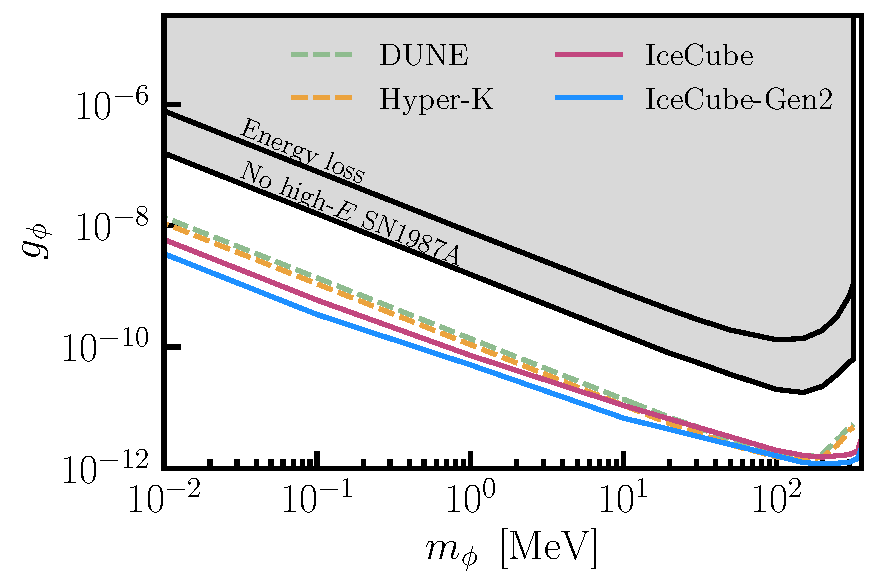
\includegraphics[width=0.47\textwidth]{figures/majoran_sensitivity}
    \caption{\textbf{\textit{Exclusion sensitivities for the Majoron case.}}
    The lines on this plot show the exclusion sensitivity for IceCube, and two next-generation neutrino experiments, Hyper-Kamiokande and DUNE.
    Additionally, we also show the reaches by SN cooling (blue) and by the lack of observation of high-energy neutrinos from SN1987A (grey) \cite{Fiorillo:2022cdq}, with the width of the shading region quantifying uncertainties from SN modeling.
    }
    \label{fig:sensitivity}
\end{figure} 
Following our strategies above, we obtain the expected exclusion limit for various BSM if no excess of hits on top of those from background noise and the standard neutrino flux were observed. The expected exclusion limit are presented in \cref{fig:sensitivity} for the Majoron case. To illustrate the broad physics application of the analysis, we also show results for the sterile neutrino case with magnetic portal in the Supplemental Materials. Current limits \cite{Fiorillo:2022cdq} from the energy loss requirement (blue band), and non-observation of high energy neutrinos from SN 1987A (gray band) are also shown in \cref{fig:sensitivity} for the Majoron case. 
With future SN explosion, IceCube can improve existing limits by one orders of magnitude. Moreover, while existing limits from time-integrated observables follow the behavior of $g_\phi\propto m^{-1}_\phi$ as Majoron production rate is proportional to $(g_\phi m_\phi)^2$, IceCube can provide stronger limit than this by focusing on the time window, especially before the peak of SM $\bar{\nu}_e$ fluxes, to reduce SM condemnations.

We also present the estimated reaches of DUNE and Hyper-K in \cref{fig:sensitivity} by looking for time-integrated high energy neutrinos following \cite{Fiorillo:2022cdq, Brdar:2023tmi}. We observe that while for the intermediate mass region, the constraints from IceCube are comparable to that from DUNE and Hyper-K, at both low mass region $m_\phi \lesssim \unit[10]{MeV}$ and high mass region $m_\phi \gtrsim \unit[200]{MeV}$, IceCube can provide stronger constraints. This is the outcome we expect. For light $\phi$ case with negligible time delay, IceCube would observe early signals in a time window separated from that when most of SM flux contribution appears, as we show in the left panel of \cref{fig:hits_and_likelihood}, thus enhancing the reaches. On the high mass end, neutrino signals will arrive much later than the SM case, where a time window at late time can be considered to reduce the standard neutrino contaminations. 

Uncertainties on the analysis from different modeling SN explosions are minor, as studied in \cite{li2023old} and potential discrepancies between data and modeling are unresolved questions.
Nevertheless, we point out that the discrepancy could be within $2\sigma$ level which will only change our exclusion limit by a small factor. We also provide the code used in this work so that the impact of SN modeling uncertainties on the sensitivity of neutrino telescopes may be evaluated in the future.

In this work, we have demonstrated that neutrino telescope such as IceCube can provide unprecedented probes of new physics, such as Majoron neutrinos and sterile neutrinos with magnetic portal, via measuring Supernova time profiles to a window as short as $\mathcal{O}(0.01)$ s. Signatures outside the SM neutrino time window, including both early and delayed signals, can be effectively probed at neutrino telescope.
This analysis can also be extended to probing new particles such as sterile neutrinos with mixing portal where the resulting time profile requires more dedicated studies as resonant conversions can happen. 

\begin{acknowledgments}
We would like to thank Thomas Janka and Daniel Kresse for providing the data from Garching core collapse SN simulations in machine-readable form, and also for stimulating discussions. Y.-Y. L is supported by the NSF of China through Grant No. 12305107, 12247103.
\end{acknowledgments}
